\documentclass{article}
%\usepackage{times}
%\usepackage{fixltx2e}
\usepackage[top=1in, bottom=1in, left=1in, right=1in]{geometry}
\usepackage[pdftex]{hyperref}
\usepackage{xargs}                      % Use more than one optional parameter in a new commands
\usepackage[pdftex,dvipsnames]{xcolor}  % Coloured text etc.
\usepackage{url}
\usepackage{verbatim}
\usepackage{listings}
\usepackage{xkvltxp}
\usepackage{fixme}
\usepackage{enumerate}
\usepackage{enumitem}
\usepackage{graphicx}
\usepackage{balance}
\usepackage{dblfloatfix}
\usepackage[skip=0pt,textfont={small,it,bf},labelfont={small,bf}]{caption}
%\usepackage{fancyhdr}
\usepackage{xspace}
\usepackage{subfigure}
\usepackage{filecontents}
\usepackage{pbox}

% tight lists
\newenvironment{tight_itemize}{
\begin{itemize}[noitemsep,leftmargin=.2in,topsep=0.in]
  \setlength{\parskip}{0pt}
  \setlength{\parsep}{0pt}
}{\end{itemize}}

\newenvironment{tight_enumerate}{
\begin{enumerate}[noitemsep]
  \setlength{\parskip}{0pt}
  \setlength{\parsep}{0pt}
}{\end{enumerate}}

\definecolor{darkgreen}{rgb}{0,0.5,0}
\definecolor{darkblue}{rgb}{0,0,0.5}
\definecolor{blue}{rgb}{0,0,0.85}
\definecolor{darkred}{rgb}{0.5,0,0}
\definecolor{gray}{rgb}{0.95,0.95,0.95}

\lstset{% general command to set parameters for the listings package
    language=c++,
        %basicstyle=\scriptsize\ttfamily,      % print entire listing as small.
        keywordstyle=\color{blue}\bfseries\ttfamily,
        identifierstyle=\ttfamily,
        commentstyle=\color{darkgreen}\itshape\ttfamily,
        showstringspaces=false,
        backgroundcolor=\color{gray},
        frame=single,               % adds a frame around the code
    tabsize=2,                      % sets default tabsize to 2 spaces
    captionpos=b,                   % sets the caption-position to bottom
    breaklines=true,                % sets automatic line breaking
    emphstyle=\color{darkred}\bfseries\sffamily,
    morekeywords={uniform,mesh,cells,vertices,edges,float3,of,forall,renderall},
}


\newcommand{\kbf}[1]{\textcolor{blue}{[kbf: #1]}}

\newcounter{todo}
\newcommand\ToDo[1]{\refstepcounter{todo}\marginpar{\color{red}{#1}}\addcontentsline{todo}{subsection}{#1~\thetodo}}%


\makeatletter
\newcommand\todoname{todo}
\newcommand\listtodoname{List of todos}
\newcommand\listoftodos{%
  \section*{\listtodoname}\@starttoc{tod}}
\makeatother

%\setlength{\belowcaptionskip}{-8pt}  % Make up a bit of space after figures. 

\begin{document}

\title{Supporting Persistent Storage within Legion}
\maketitle

\section{High level overview}
To support persistent storage within Legion we will model file(s) or object(s) in permanent
storage as a physical instance of a logical region. This model is consistent
with the overall design of Legion, borrowing the concept of a physical region
that is traditionally backed by memory and extending this to physical regions
that will be backed by storage. To guarantee consistency we will place the
restriction of restricted access mode on storage backed physical regions. The
implication of which is that the application will have to manage concurrent
access to the logical region via acquire/release semantics. More information
on restricted access can be found
in \url{http://legion.stanford.edu/pdfs/bootcamp/06_advanced_features.pdf} and
\url{http://legion.stanford.edu/tutorial/ghost.html}.


The restricted mode of access allows concurrent access with
application/user-level software coherence management. Coherence is
accomplished through he use of acquire/release of whole or part of the
physical region.

\textbf{Add a more
  complete discussion on the implications of restricted access
  here.}\ToDo{Galen}

\section{Interfaces}
To model files/objects in permanent storage as a physical instance of a
logical region we introduce a 
To instantiate a physical region that is backed by an HDF5 file on permanent
storage we introduce the \lstinline{runtime->map_hdf member} function.
\begin{lstlisting}
  PhysicalRegion hdf5_pr = runtime->map_hdf(Context ctx,
                                            char* file_name,
                                            LogicalRegion logical_region,
                                            std::map<FieldID,
                                            HDF5PathName>fields_set,
                                            legion_file_mode_t mode)
  
\end{lstlisting}

\begin{tight_itemize}
  
\item \lstinline{char* file_name} :  specifies the
  full path to the HDF5 file

\item \lstinline{LogicalRegion logical_region} :
  specifies the logical region that is associated with the HDF5 file. The HDF5
  file on disk must have the same index space as the logical region, Legion
  will check this constraint. \textbf{What error or exception is raised if
    this isn't the case?} \ToDo{Zhihao}
  
\item \lstinline{ std::map<FieldID, char * HDF5PathName> fields_set} :
  Mapping between Legion FieldID and the HDF5PathName to the
  dataset. HDF5PathName is the fully qualified path name including group(s)
  and dataset name. 
  The HDF5 dataset type must match the field type in Legion and the dimension
  of the dataset must match the index space dimension in Legion.
  \textbf{What error or exception is raised 
    if this isn't the case} \ToDo{Zhihao} 

\item \lstinline{ legion_file_mode_t} : The file access mode, valid modes are:
  \lstinline{FILE_EXCL, FILE_TRUNC, FILE_READ_ONLY, FILE_READ_WRITE}
  Note that region access must be consistent with these modes and it is
  considered a program error to open a file in \lstinline{FILE_READ_ONLY}
  mode and then write to physical region. 
  
\item Return value \lstinline{PhysicalRegion hdf5_pr}: a Legion physical region 
 
\end{tight_itemize}

\begin{figure}[hhh]
  \centering 
  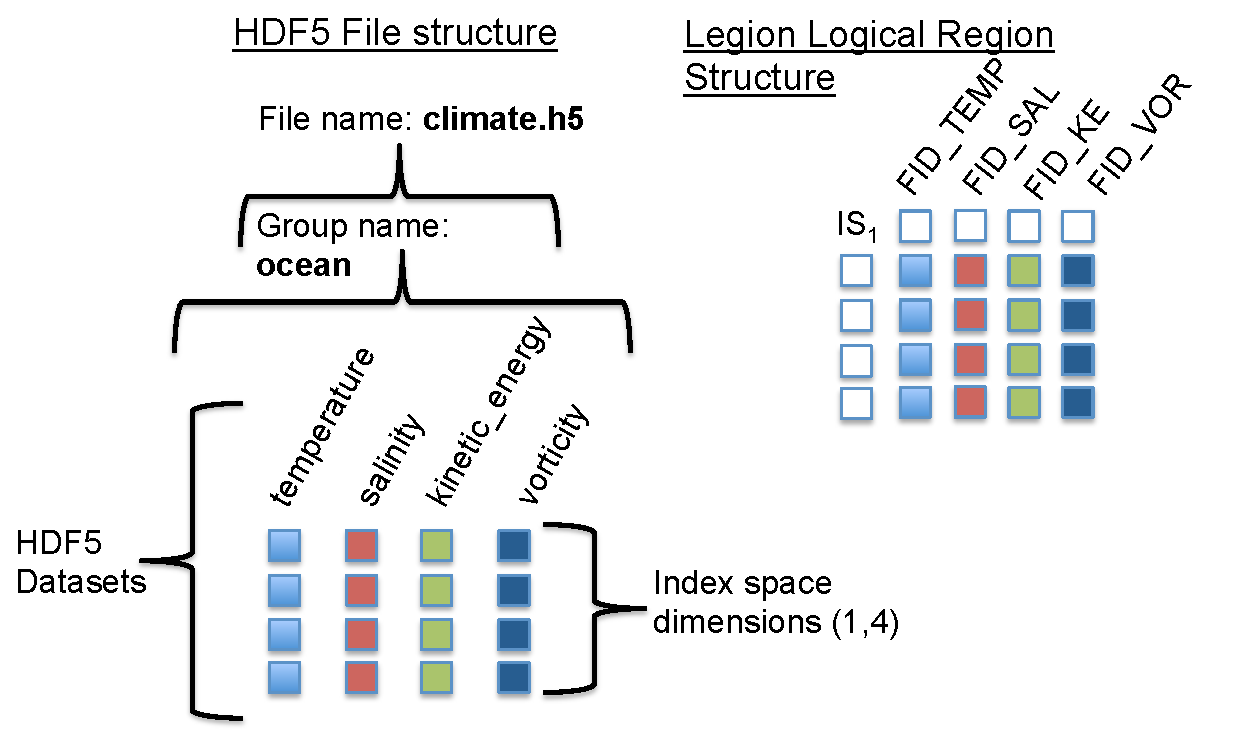
\includegraphics[width=0.8\textwidth]{figs/hdf5-layout-climate.pdf}
  \caption{Example HDF5 file structure and corresponding Legion logical region} 
  \label{figure:hdf5layout-climate}
\end{figure}


File access modes and there effects are
\begin{itemize}
  \item \lstinline{FILE_EXCL}: If the file already exists, \lstinline{map_hdf}
    fails. If the file does not exist, it is created and opened with
    read-write access
  \item \lstinline{FILE_TRUNC}: If the file already exists, the file is opened
    with read-write access, and new data will overwrite any existing data. If
    the file does not exist, it is created and opened with read-write
    access. If the file exists, datasets specified in \lstinline{fields_set} 
    will be verified to exist and index space bounds are checked and an
    exception raised if failure. If the file does not exist, the datasets (and
    group(s)) specified in
    \lstinline{fields_set} are created with the index space specified in
    the logical region.
  \item \lstinline{FILE_READ_ONLY}: An existing file is opened with read-only
    access. Datasets, and index space bounds are checked.  If the
    file does not exist an exception is raised. Subsequent 
    attempts to write to the physical region are 
    invalid. \textbf{Can we return an error or raise an exception if this
      occurs? Do we have enough context to know that the file was opened
      read-only?}
    \ToDo{Zhihao}
  \item \lstinline{FILE_READ_WRITE}: An existing file is opened with
    read-write access. If the file does not exist an exception is
    raised. Datasets, and index space bounds are checked.  
\end{itemize}


The \lstinline{map_hdf} operation invalidates all existing physical instances
associated with the \lstinline{fields_set} within
\lstinline{logical_region}, which makes the HDF5 file the only valid
physical instance of the logical region. This is for consistency as Legion
cannot guarantee that data in the HDF5 file is always consistent with existing
in-memory instances. Restricted access mode is designed for this purpose
assuring that copies of the region are not instantiated by the Legion
runtime.

Once the file/object is mapped to a logical region, the physical region may be
acted on like any other physical region (within the constraints of restricted
access mode) with all expected Legion operations.


\begin{lstlisting}
  void unmap_region (Context ctx, PhysicalRegion region)
\end{lstlisting}

Unmapping a physical region closes the file and invalidates
\lstinline{PhysicalRegion region}. 

\section{Uses of this interface}

\subsection{Mapping an existing HDF5 file}

The following is a an example of using the \lstinline{map_hdf} method to
open an existing HDF5 file as illustrated in
Figure~\ref{figure:hdf5layout-climate}. 
\begin{lstlisting}
 Rect<1> elem_rect(Point<1>(0), Point<1>(3));

 IndexSpace is = runtime->create_index_space(ctx,
                                             Domain::from_rect<1>(elem_rect));
 
 enum FieldIDs {
     FID_TEMP,
     FID_SAL,
     FID_KE,
     FID_VOR
 }
 
 FieldSpace fs = runtime->create_field_space(ctx);
 {
     FieldAllocator allocator = create_field_allocator(ctx, fs);
     allocator.allocate_field(sizeof(double), FID_TEMP);
     allocator.allocate_field(sizeof(double), FID_SAL);
     allocator.allocate_field(sizeof(double), FID_KE);
     allocator.allocate_field(sizeof(double), FID_VOR);
 }
 
 LogicalRegion ocean_lr = runtime->create_logical_region(ctx, is, fs);
 
 std::map<FieldID, char*> fields_map;
 fields_map[FID_TEMP] = “/ocean/temperature”;
 fields_map[FID_SAL] = “/ocean/salinity”;
 fields_map[FID_KE] = “/ocean/kinetic_energy”;
 fields_map[FID_VOR] = “/ocean/vorticity”;
 
 
 PhysicalRegion hdf5_climate = runtime->map_hdf(ctx, “./climate.h5”,
                                                ocean_lr, fields_map,
                                                FILE_READ_WRITE);
 
 \end{lstlisting}

 \subsection{Directly accessing the HDF5 file with a region accessor}
 \begin{lstlisting}
 RegionAccessor<AccessorType::Generic> acc_ocean =
     hdf5_climate.get_field_accessor(FID_TEMP).typeify<double>();
 
 Domain dom = runtime->get_index_space_domain(ctx,
                                              ocean_lr.get_index_space());
 Rect<1> rect = dom.get_rect<1>();
 
 
 double temps[4];
 double temp = temps;
 for(GenericPointInRectIterator<1> pir(rect); pir; pir++) { 
     *temp = acc.read(DomainPoint::from_point<1>(pir.p));
     temp++; 
 }
 
 for(GenericPointInRectIterator<1> pir(rect); pir; pir++) {
     acc.write(DomainPoint::from_point<1> (pir.p), temp);
     temp--;
 }
 
 runtime->unmap_region(ctx, hdf5_climate);
 \end{lstlisting}
 
 \subsection{Copy HDF5 fields to other fields mapped in fast memory}
 
 \begin{lstlisting}
 Rect<1> elem_rect(Point<1>(0), Point<1>(3));

 IndexSpace is = runtime->create_index_space(ctx,
                                             Domain::from_rect<1>(elem_rect));
 
 enum FieldIDs {
     FID_TEMP,
     FID_SAL,
     FID_KE,
     FID_VOR,
     FID_TEMP_FM,
     FID_SAL_FM,
     FID_KE_FM,
     FID_VOR_FM
 
 }
 
 FieldSpace fs = runtime->create_field_space(ctx);
 {
     FieldAllocator allocator = create_field_allocator(ctx, fs);
     allocator.allocate_field(sizeof(double), FID_TEMP);
     allocator.allocate_field(sizeof(double), FID_SAL);
     allocator.allocate_field(sizeof(double), FID_KE);
     allocator.allocate_field(sizeof(double), FID_VOR);
     allocator.allocate_field(sizeof(double), FID_TEMP_FM);
     allocator.allocate_field(sizeof(double), FID_SAL_FM);
     allocator.allocate_field(sizeof(double), FID_KE_FM);
     allocator.allocate_field(sizeof(double), FID_VOR_FM);
     
 }
 
 LogicalRegion ocean_lr = runtime->create_logical_region(ctx, is, fs);
 
 std::map<FieldID, char*> fields_map;
 fields_map[FID_TEMP] = “/ocean/temperature”;
 fields_map[FID_SAL] = “/ocean/salinity”;
 fields_map[FID_KE] = “/ocean/kinetic_energy”;
 fields_map[FID_VOR] = “/ocean/vorticity”;
 
 
 PhysicalRegion hdf5_climate = runtime->map_hdf(ctx, “./climate.h5”,
                                                ocean_lr, fields_map,
                                                FILE_READ_WRITE);


 RegionRequirement req(ocean_lr, READ_WRITE, EXCLUSIVE, ocean_lr);
 req.add_field(FID_TEMP_FM);
 req.add_field(FID_SAL_FM);
 req.add_field(FID_KE_FM);
 req.add_field(FID_VOR_FM);
 InlineLauncher ocean_launcher(req);

 PhysicalRegion ocean_pr = runtime->map_region(ctx, ocean_launcher);
 ocean_pr.wait_until_valid();


 \\ need more here.. 
 
 \end{lstlisting}
 

 
 \textbf{We need fleshed out examples here}
 
 
 \section{Implementation}
 The current implementation of persistent storage within Legion abstracts the
file/object as a locally accessible physical region, similar to a physical
memory. The implication of this design is that file/object I/O is serialized
to a single owner of physical region and all other tasks will coordinate
access through this single owner. In some cases this is required as the
file/object storage namespace is not globally accessible and will need to be
treated as a node-level resource similar to a physical memory. In other cases,
the file/object will be globally accessible to all nodes such as in a
networked file system, parallel file system, or key/value store
environment. In these cases, access to the file/object could be direct from
each node in the system, and is similar in spirit to a GASNet based memory in
the current Legion implementation.

In the next iteration of the design we will need to accommodate global
namespaces allowing each node to directly access the file/object underlying a
logical region. In the read-only case this can enable independent access to
the underlying file from all clients. In the read-write case, this can enable
coordinated access in parallel.

\begin{enumerate}
  \item Tasks on different nodes can independently access disjoint fields
    (datasets) within the same HDF5 file. This could be achieved by using
    \lstinline{RegionRequirement::add_field}. The first task that executed
    with this region requirement would then be the task leader for this
    dataset within the HDF5 file.
  \item Tasks on different nodes can independently access disjoint partitions
    across index space in a similar fashion to disjoint fields.
\end{enumerate}

\textbf{What are the implications of this approach?} \ToDo{Zhihao, Sean, Mike,
Noah, Galen}



\textbf{One current issue is that concurrent (independent or parallel) access
  must use the PHDF5 interface for opening the HDF5 file}. See
  \url{https://www.hdfgroup.org/hdf5-quest.html#gconc1}


\textbf{Another issue is that HDF5 is not thread safe.}


\subsection{Future work}
We should consider how to handle sharded file/object access within
Legion. This fits well with partitioned logical regions in that each disjoint
region within a partition could be saved as a separate file/object within the
file system. We would need to have some metadata describing how to access
these shards, perhaps an index/partition file that held the region tree
information and the mapping to individual shards. \textbf{More to come} \ToDo{Galen} 

\end{document}
